\documentclass{ctexart}
\usepackage{graphicx} % Required for inserting images
\usepackage{hyperref}
\usepackage{float}
\usepackage{listings}
\usepackage{xcolor}
\usepackage{multirow}
\usepackage{multicol}
\usepackage{booktabs}
\usepackage{amsmath}
\usepackage[letterpaper,top=2cm,bottom=2cm,left=3cm,right=3cm,marginparwidth=1.75cm]{geometry}

\hypersetup{
    colorlinks=true,
    linkcolor=blue,
    filecolor=blue,
    urlcolor=blue,
    citecolor=cyan,
}

\definecolor{codegreen}{rgb}{0,0.6,0}
\definecolor{codegray}{rgb}{0.5,0.5,0.5}
\definecolor{codepurple}{rgb}{0.58,0,0.82}
\definecolor{backcolour}{rgb}{0.95,0.95,0.92}

\lstdefinestyle{mystyle}{
    backgroundcolor=\color{backcolour},
    commentstyle=\color{codegreen},
    keywordstyle=\color{magenta},
    stringstyle=\color{codepurple},
    basicstyle=\ttfamily\footnotesize,
    breakatwhitespace=false,
    breaklines=true,
    captionpos=b,
    keepspaces=true,
    showspaces=false,
    showstringspaces=false,
    showtabs=false,
    tabsize=2
}
\lstset{style=mystyle}

\title{EIEN6023P:Lab2-有限状态机实验}
\author{}
\date{}

\begin{document}

\maketitle

\section{实验目标}
\begin{itemize}
    \item 学习Mealy有限状态机和Moore有限状态机的结构
    \item 学习状态机的Verilog两段式和三段式写法
    \item 设计一个有限状态机来控制交通信号灯
    \item 使用Verilog实现所设计的有限状态机
    \item 在FPGAOL平台上进行验证所编写的代码
\end{itemize}

%------------------------------%

\section{有限状态机}

逻辑电路可以分为两大类:“组合”逻辑电路和“时序”逻辑电路。前面您已经学习组合逻辑电路,其输出只取决于当前的输入。时序逻辑电路的输出不仅取决于当前的输入,而且取决于过去的输入序列,这个序列是任意长的。

对于组合逻辑电路,可以通过输入输出之间的\textbf{真值表}来描述其功能。而对于时序逻辑电路,使用真值表描述其功能是不现实的,无法确定需要取一个多长的输入组合取值序列,因此时序逻辑电路一般采用\textbf{有限状态机}作为电路行为的描述。

有限状态机主要由数量有限的状态和状态之间的转换规则组成。数字逻辑电路中的状态变量都是二进制数值,对应着电路中的某些逻辑信号。如交通信号灯电路中,不同信号灯的亮灭可以使用数个二进制值来表示。时序电路的状态变化大多依靠时钟信号来规定,在时钟的边沿,状态机根据规则转换当前的状态。

\subsection{D触发器}

大多数时序电路均采用D触发器来存储它们的状态变量,上升沿触发的D触发器逻辑符号和功能表如图所示。

\begin{figure}[H]
    \centering
    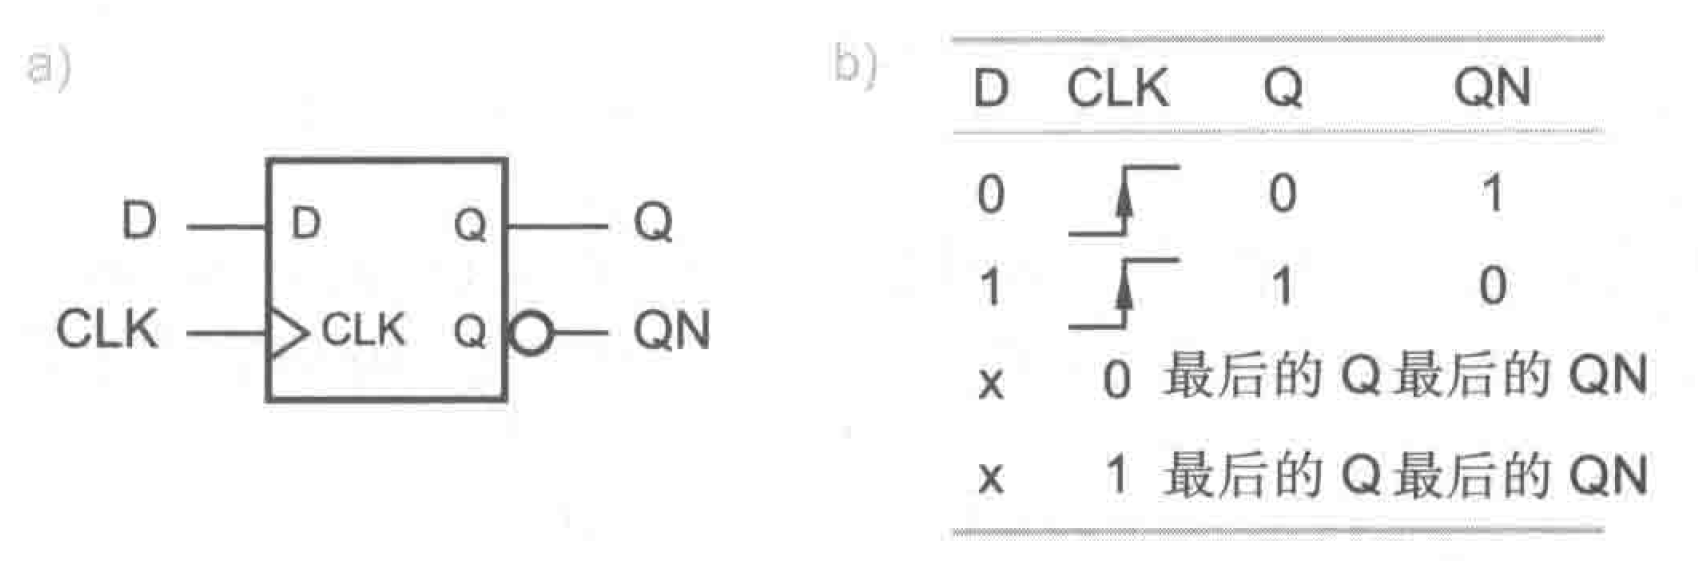
\includegraphics[width=0.6\textwidth]{lab2/1.png}
\end{figure}

电路的输入是数据信号D和时钟信号CLK,输出为Q以及可选的QN(Q补)。当CLK从低电平转换到高电平时,电路对D进行采样,并把Q置为当前D的值(QN置为D的反)。上述CLK从低电平到高电平的变化期间,Q(以及QN)的值保持不变。下图展示了一个上升沿触发的D触发器针对所举例的输入序列的功能特性。

\begin{figure}[H]
    \centering
    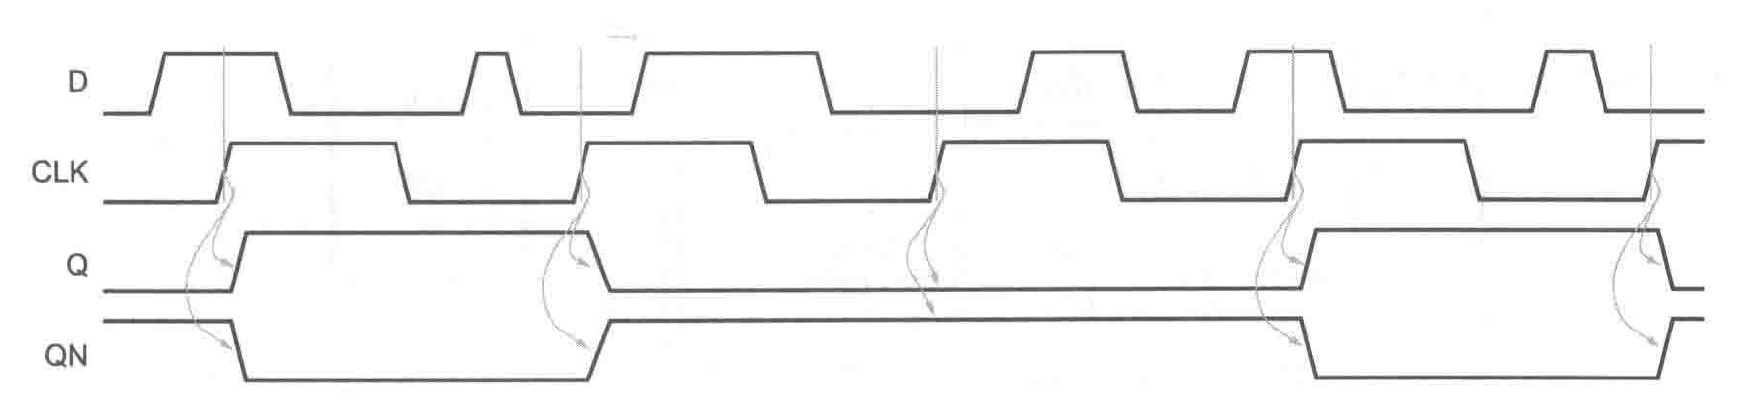
\includegraphics[width=\textwidth]{lab2/2.png}
\end{figure}

在Verilog中可以使用行为建模对正边沿触发的D触发器建模,如下所示。

\begin{lstlisting}[language=Verilog]
module D_ff_behavior (input D, input CLK, output reg Q); 
    always @ (posedge CLK)
        Q <= D;
endmodule
\end{lstlisting}

\subsection{Mealy有限状态机和Moore有限状态机}

图1与图2给出了两种常用状态机的结构,主要由三部分构成。图中的“当前状态时序逻辑”是存储当前状态的$n$个触发器,可用于表达$2^n$种状态。状态机中的所有触发器都由一个公共的时钟信号驱动,在时钟信号的触发沿(上升沿或下降沿)上改变其状态。状态机状态(即触发器的值)由“下一状态转移组合逻辑$F$"的输出决定,该组合逻辑$F$接收当前状态和当前输入作为状态转移判断。电路输出由“输出组合逻辑$G$”来决定,根据该组合逻辑$G$\textbf{是否接收输入信号},可以将状态机分为\textbf{Mealy机}和\textbf{Moore机}两种,如图1与图2所示。

\begin{figure}[H]
    \centering
    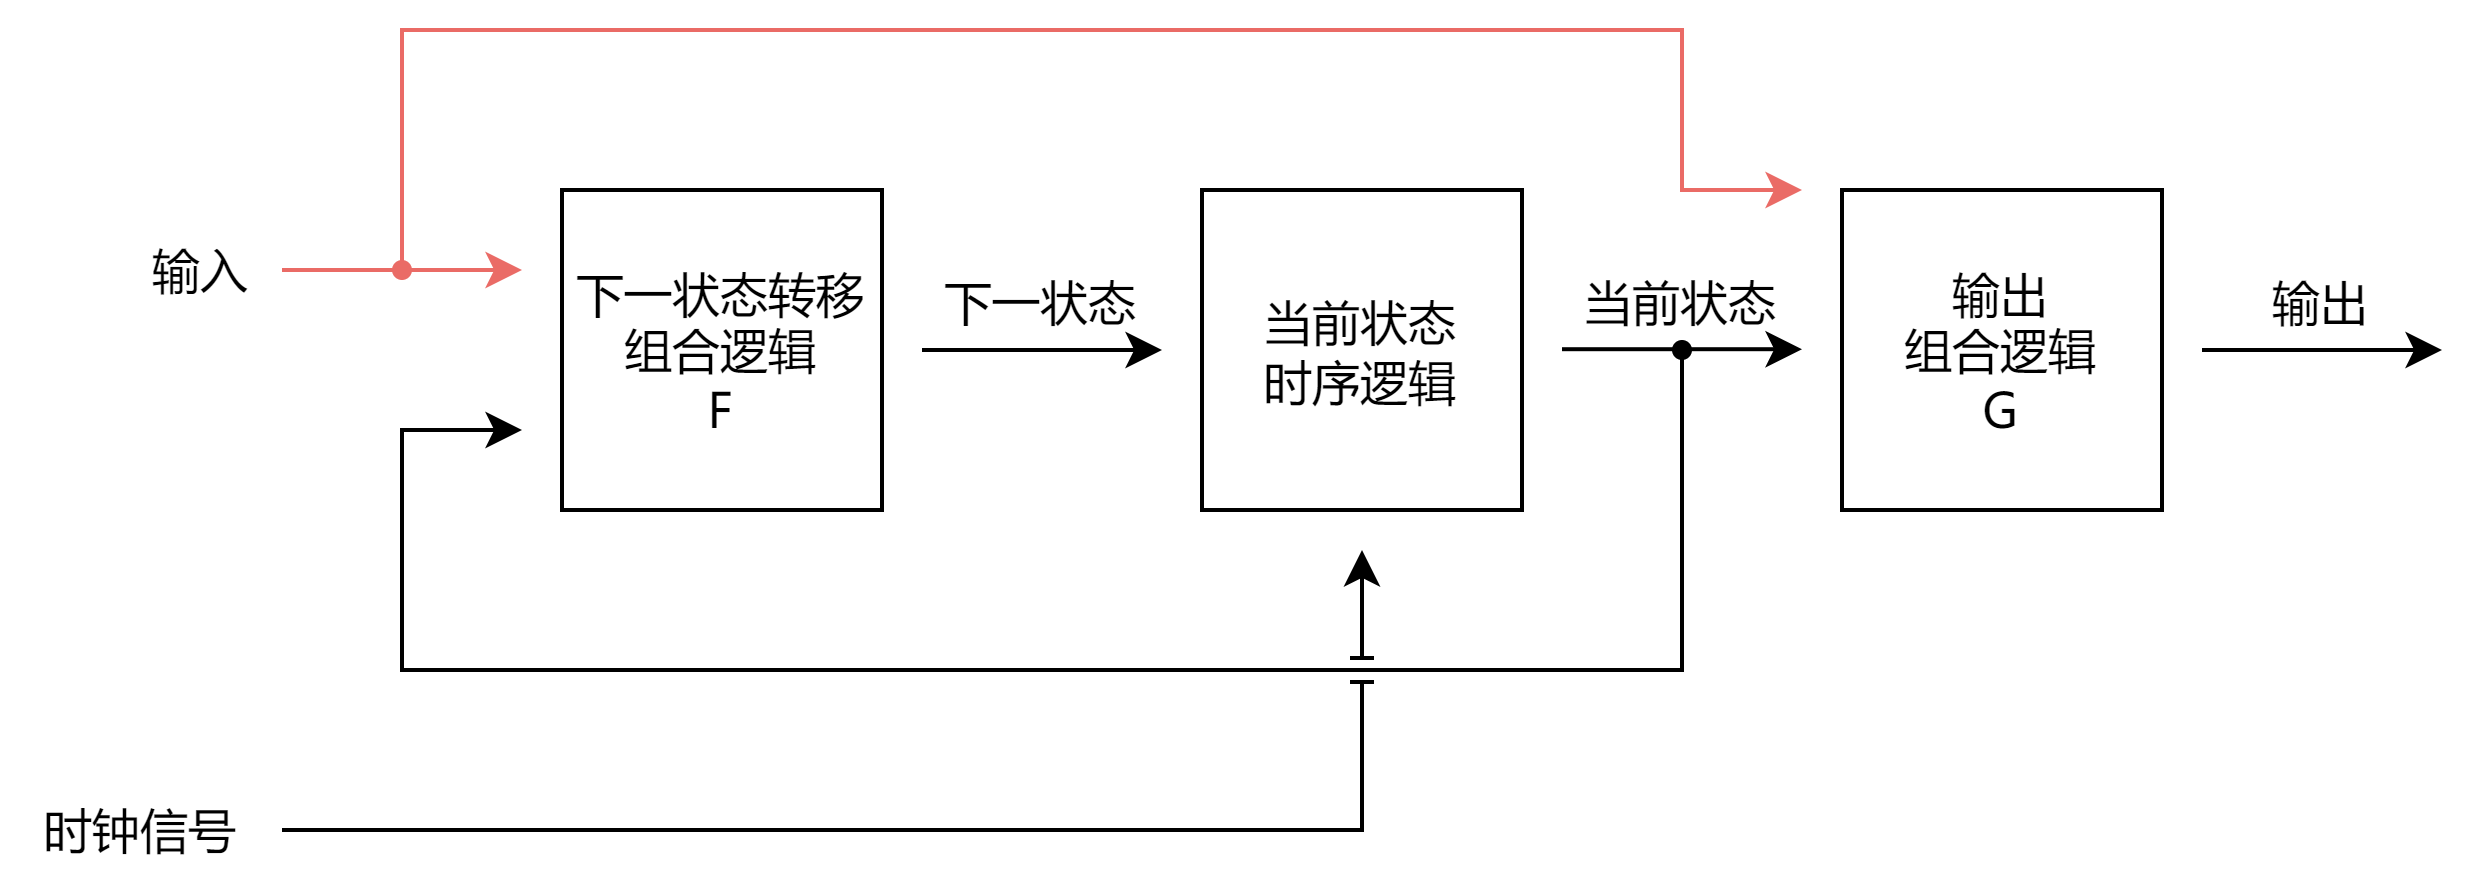
\includegraphics[width=0.8\textwidth]{lab2/3.png}
    \caption{Mealy机:$下一状态=F(当前状态,输入)$,$输出=G(当前状态,输入)$}
\end{figure}

\begin{figure}[H]
    \centering
    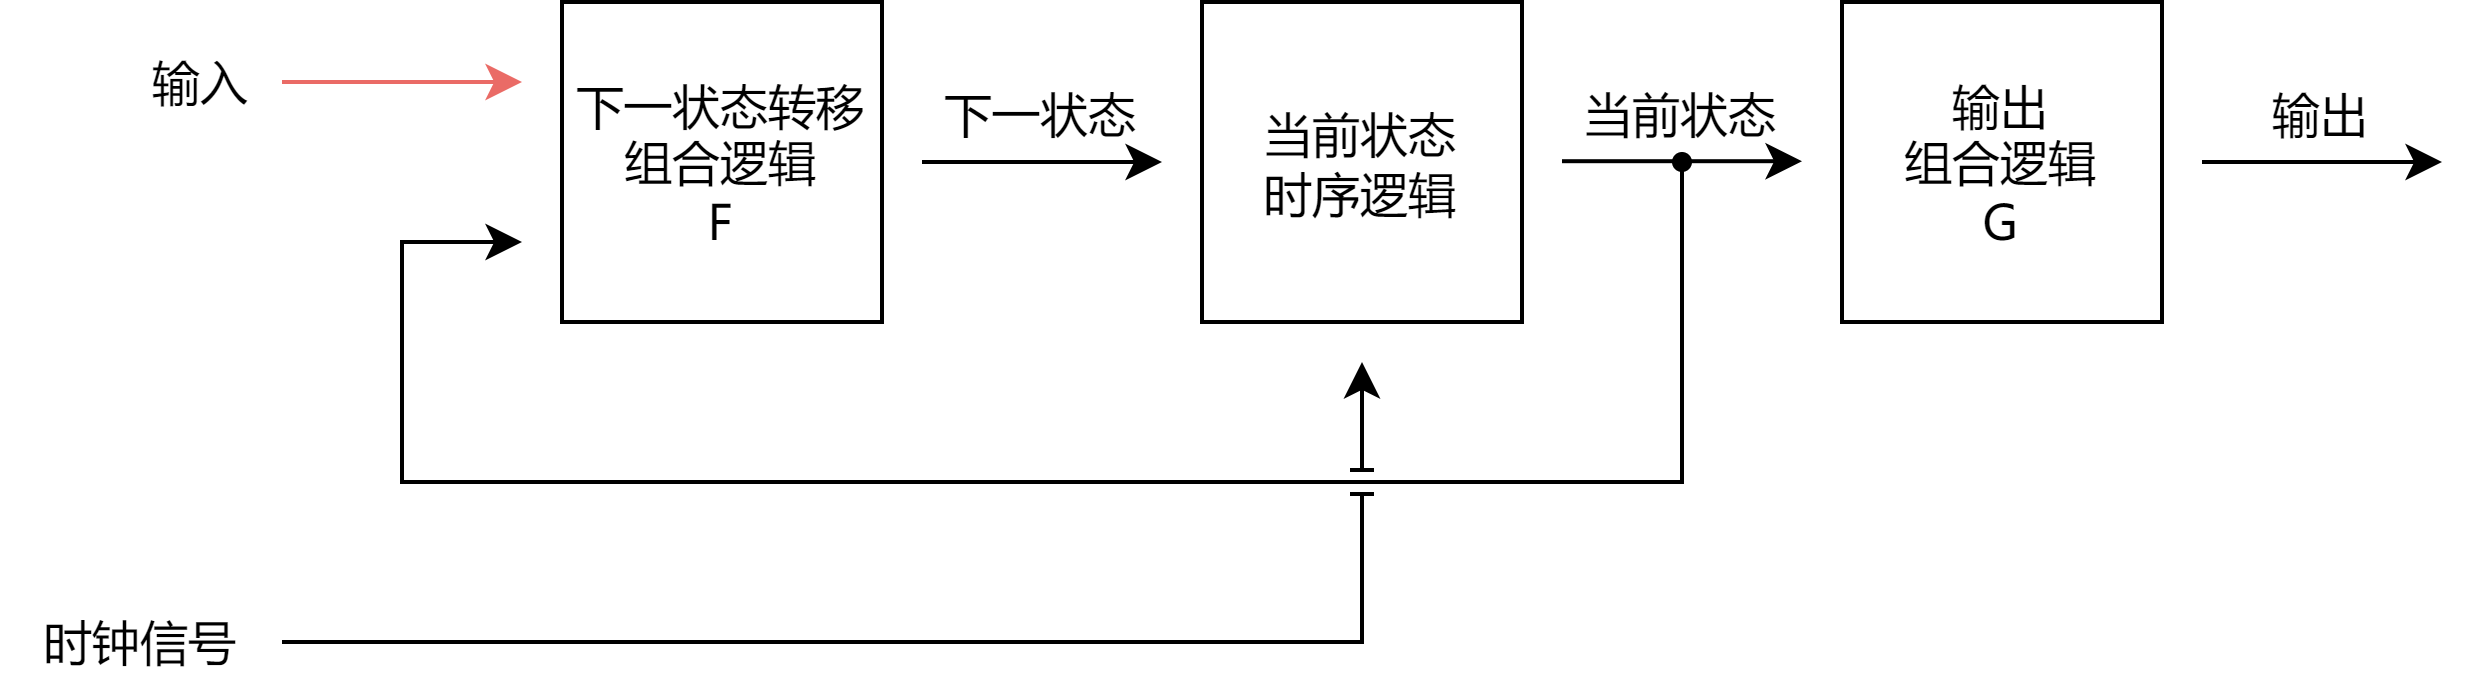
\includegraphics[width=0.8\textwidth]{lab2/4.png}
    \caption{Moore机:$下一状态=F(当前状态,输入)$,$输出=G(当前状态)$}
\end{figure}

Mealy机和Moore机拥有各自的优缺点,在实际的电路设计中都有可能被使用。由于Mealy机可以由当前输入直接得到输出结果而不经过状态转换,因此在实现相同功能时,Mealy机可以比Moore机少一个状态,而且Mealy机的输出可以比Moore机提前一个时钟周期。但由于Mealy机的输出可能由当前输入得出,因此系统的输出容易受到输入信号中的毛刺影响,如果系统不能承受这种影响,则应使用Moore机。

我们通过一个例子来更深入地理解Mealy机和Moore机的异同。下图是一个Mealy机的状态图,该状态机的作用是将输入的二进制序列转换为补码,先输入的是最低有效位。状态图中,每个节点对应着一个状态,每条有向边表示一个状态转移。由于Mealy机的输出是当前状态和输入的函数,因此Mealy机的输出被标注在每一条有向边上。

\begin{figure}[H]
    \centering
    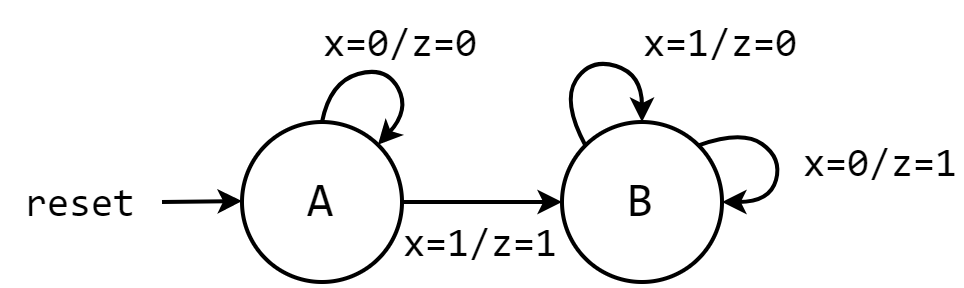
\includegraphics[width=0.5\textwidth]{lab2/5.png}
\end{figure}

\textbf{STEP1}:根据状态图,完成以下Mealy机Verilog代码填空,使之实现正确的功能。

\begin{lstlisting}[language=Verilog]
module top_mealy (input clk, input reset, input x, output z); 
    parameter A = 2'b01;
    parameter B = 2'b10;

    reg [1:0] next_state;
    reg [1:0] state;

    // comb logic to generate next state
    always @(state, x) begin
        case (state)
            A: next_state = /***** fill in this field *****/;
            B: next_state = /***** fill in this field *****/;
            default: next_state = A;
        endcase
    end

    // seq logic to generate current state
    always @(posedge clk or posedge reset) begin
        if (reset)
            state <= A;
        else
            state <= next_state;
    end

    // comb logic to generate output
    reg output_z;
    always @(state, x) begin
        case (state)
            A: output_z = /***** fill in this field *****/;
            B: output_z = /***** fill in this field *****/;
            default: output_z = 1'b0;
        endcase
    end
    assign z = output_z;

endmodule
\end{lstlisting}

如果使用Moore机来实现相同的功能,则需要新增一个中间状态,其状态图如下图所示。由于Moore机的输出与输入无关,仅由状态机当前的状态决定,因此Moore机的输出被标注在每一个节点上。

\begin{figure}[H]
    \centering
    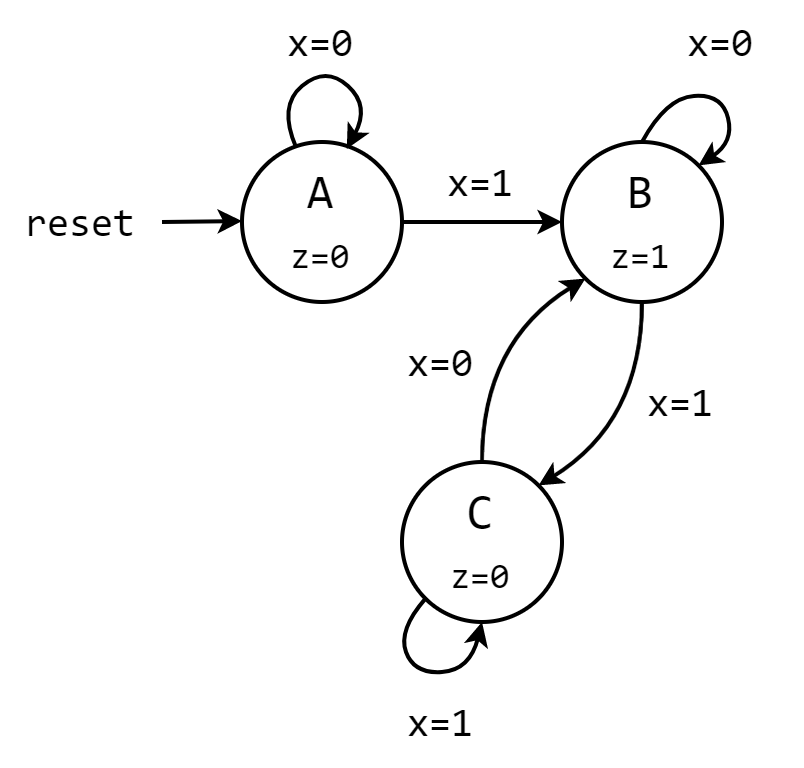
\includegraphics[width=0.45\textwidth]{lab2/6.png}
\end{figure}

\textbf{STEP2}:根据状态图,完成以下Moore机Verilog代码填空,使之实现正确的功能。
\begin{lstlisting}[language=Verilog]
module top_moore (input clk, input reset, input x, output z); 
    parameter A = 3'b001;
    parameter B = 3'b010;
    parameter C = 3'b100;
    
    reg [2:0] next_state;
    reg [2:0] state;

    // comb logic to generate next state
    always @(state, x) begin
        case (state)
            A: next_state = /***** fill in this field *****/;
            B: next_state = /***** fill in this field *****/;
            C: next_state = /***** fill in this field *****/;
            default: next_state = A;
        endcase
    end

    // seq logic to generate current state
    always @(posedge clk or posedge reset) begin
        if (reset)
            state <= A;
        else
            state <= next_state;
    end

    // comb logic to generate output
    assign z = /***** fill in this field *****/;

endmodule
\end{lstlisting}

\subsection{状态机的两段式和三段式写法}

在上一节中您已经初步学习了使用Verilog表示状态机的方法,即使用一个always块表示当前状态的时序逻辑,使用两个always块表示下一状态转移的组合逻辑F与输出的组合逻辑G。这种实现方法被称作状态机的\textbf{两段式写法},即触发器分割了两部分的组合逻辑,电路的时序路径较短,可以获得更高的性能。由于两段式写法的输出由组合逻辑给出,因此输出信号可能存在毛刺。为了解决这个问题,可以使用\textbf{三段式写法}实现状态机。

在状态机的三段式写法中,输出端会增加一级触发器一滤除输出组合逻辑G可能产生的毛刺信号,而且输出组合逻辑G是根据下一状态来对输出做出判断,这样做不会消耗多余的时钟周期。如图所示为Moore机的三段式写法的结构图。

\begin{figure}[H]
    \centering
    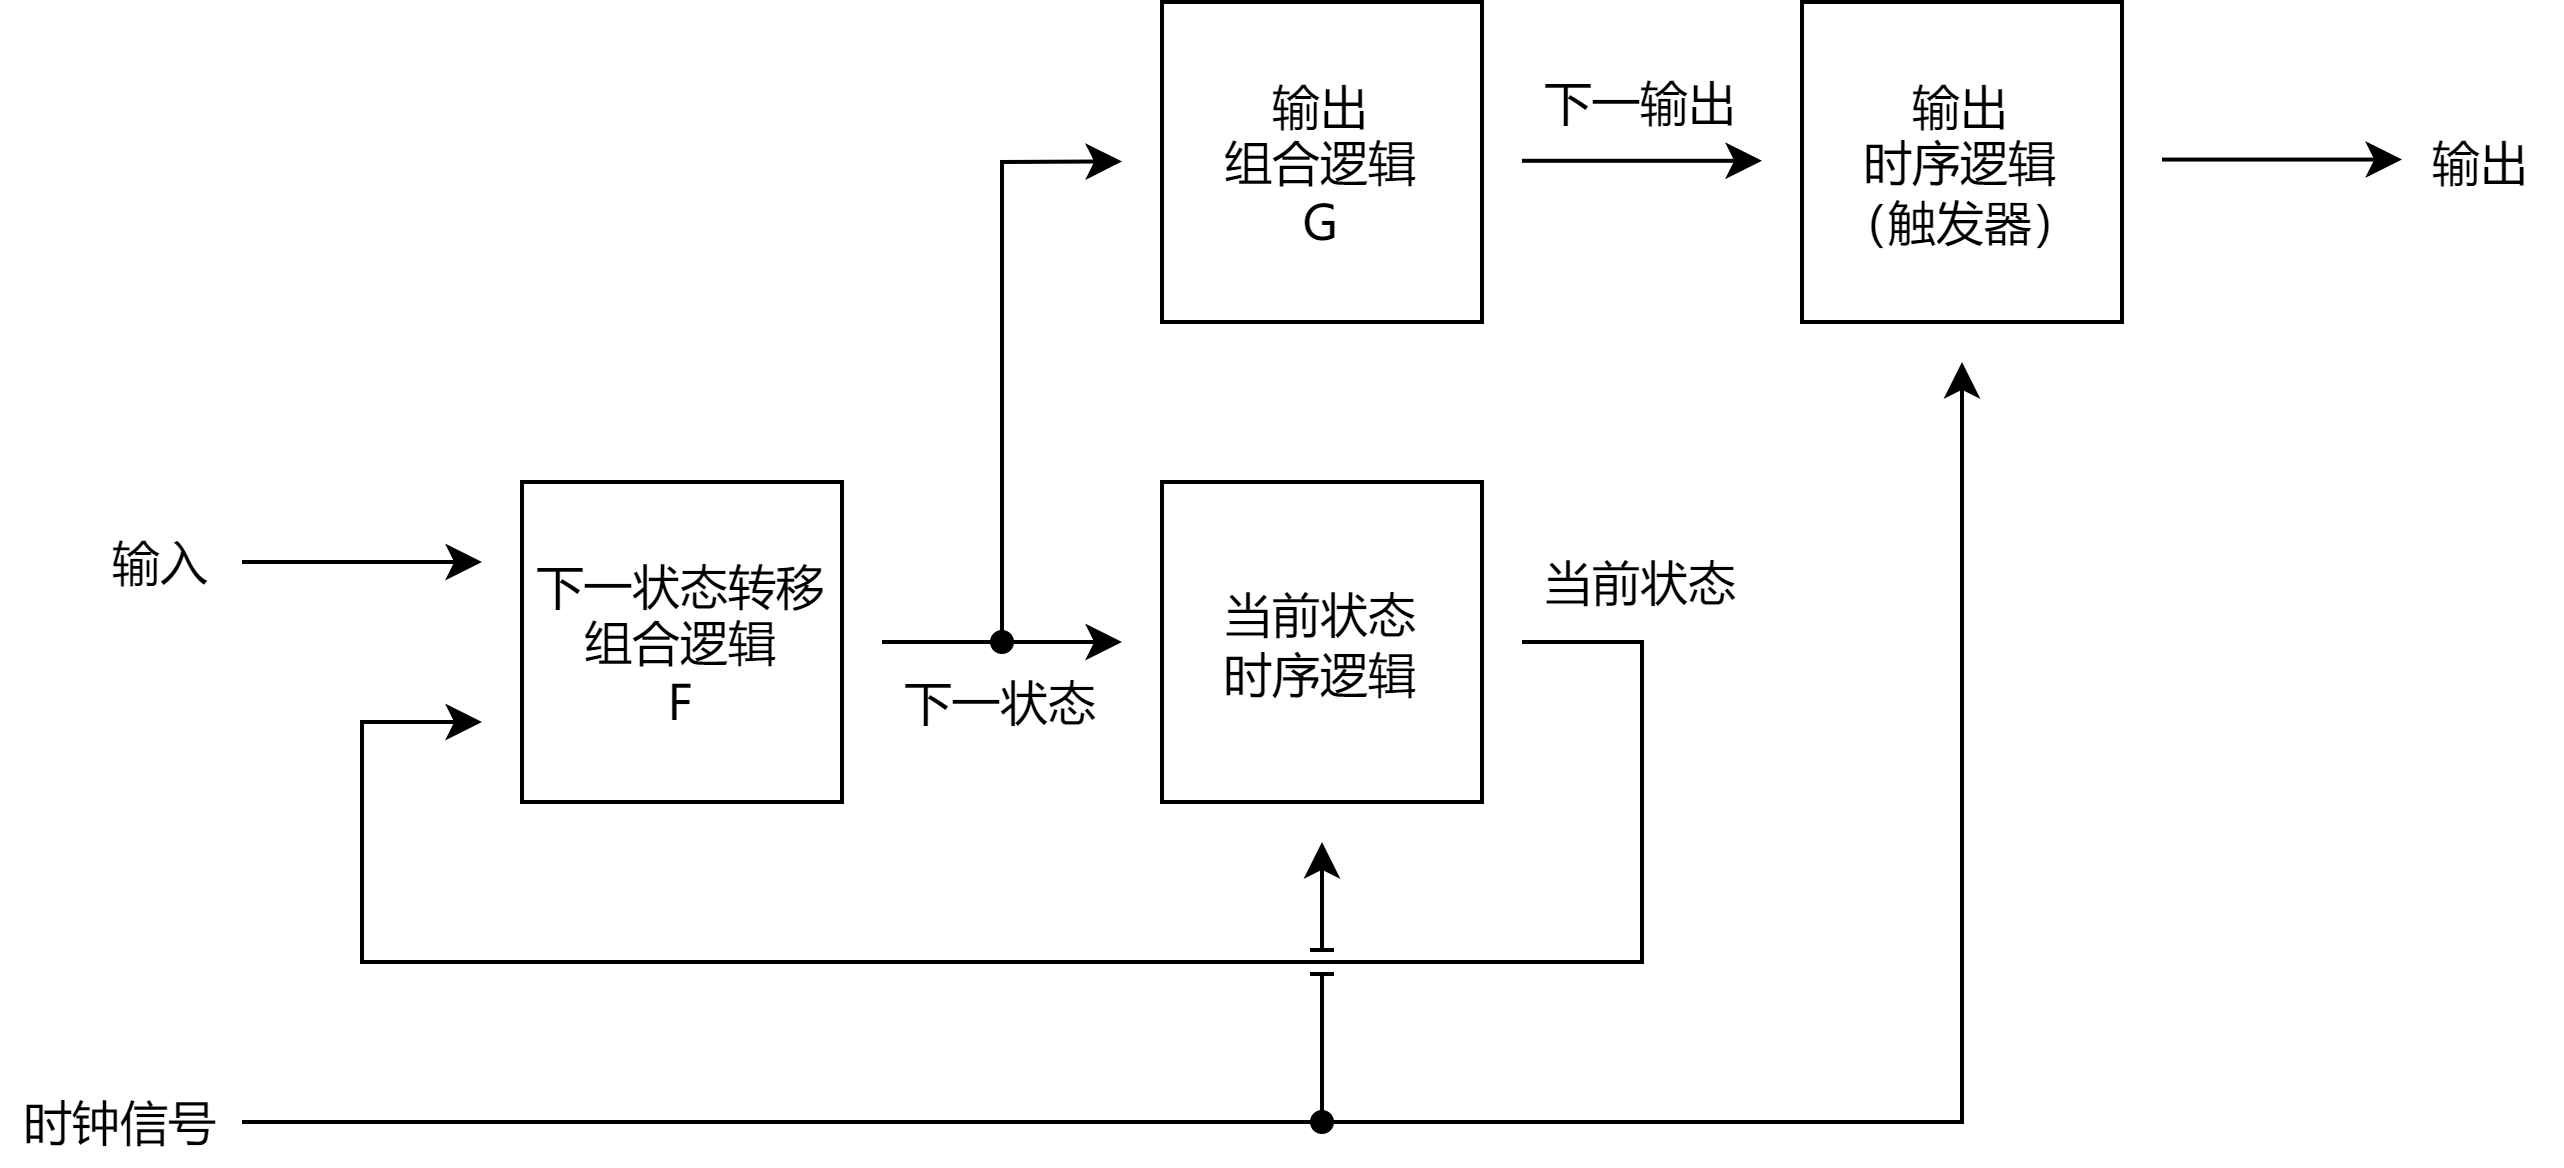
\includegraphics[width=0.8\textwidth]{lab2/7.png}
\end{figure}

\textbf{STEP3}:根据上述三段式写法的结构图,将2.2节中Moore机的两段式Verilog代码实现改为三段式,完成代码填空。
\begin{lstlisting}[language=Verilog]
module top_moore (input clk, input reset, input x, output z); 
    parameter A = 3'b001;
    parameter B = 3'b010;
    parameter C = 3'b100;

    reg [2:0] next_state;
    reg [2:0] state;

    // comb logic to generate next state
    always @(state, x) begin
        case (state)
            A: next_state = /***** fill in this field *****/;
            B: next_state = /***** fill in this field *****/;
            C: next_state = /***** fill in this field *****/;
            default: next_state = A;
        endcase
    end

    // seq logic to generate current state
    always @(posedge clk or posedge reset) begin
        if (reset)
            state <= A;
        else
            state <= next_state;
    end

    // seq logic to generate output
    reg output_z;
    always @(posedge clk or posedge reset) begin
        if (reset)
            output_z <= 1'b0;
        else
            output_z <= /***** fill in this field *****/;
    end
    assign z = output_z;

endmodule
\end{lstlisting}

那么Mealy机是否有相应的三段式写法呢?由于Mealy机的输出可能由当前输入得出,而输出的时序逻辑并不能得到下一输入,因此为了保证功能的正确性,必须在输出的时序逻辑后再增加一个组合逻辑H,以根据当前的输入计算输出。如图所示为Mealy机的三段式写法的结构图。

\begin{figure}[H]
    \centering
    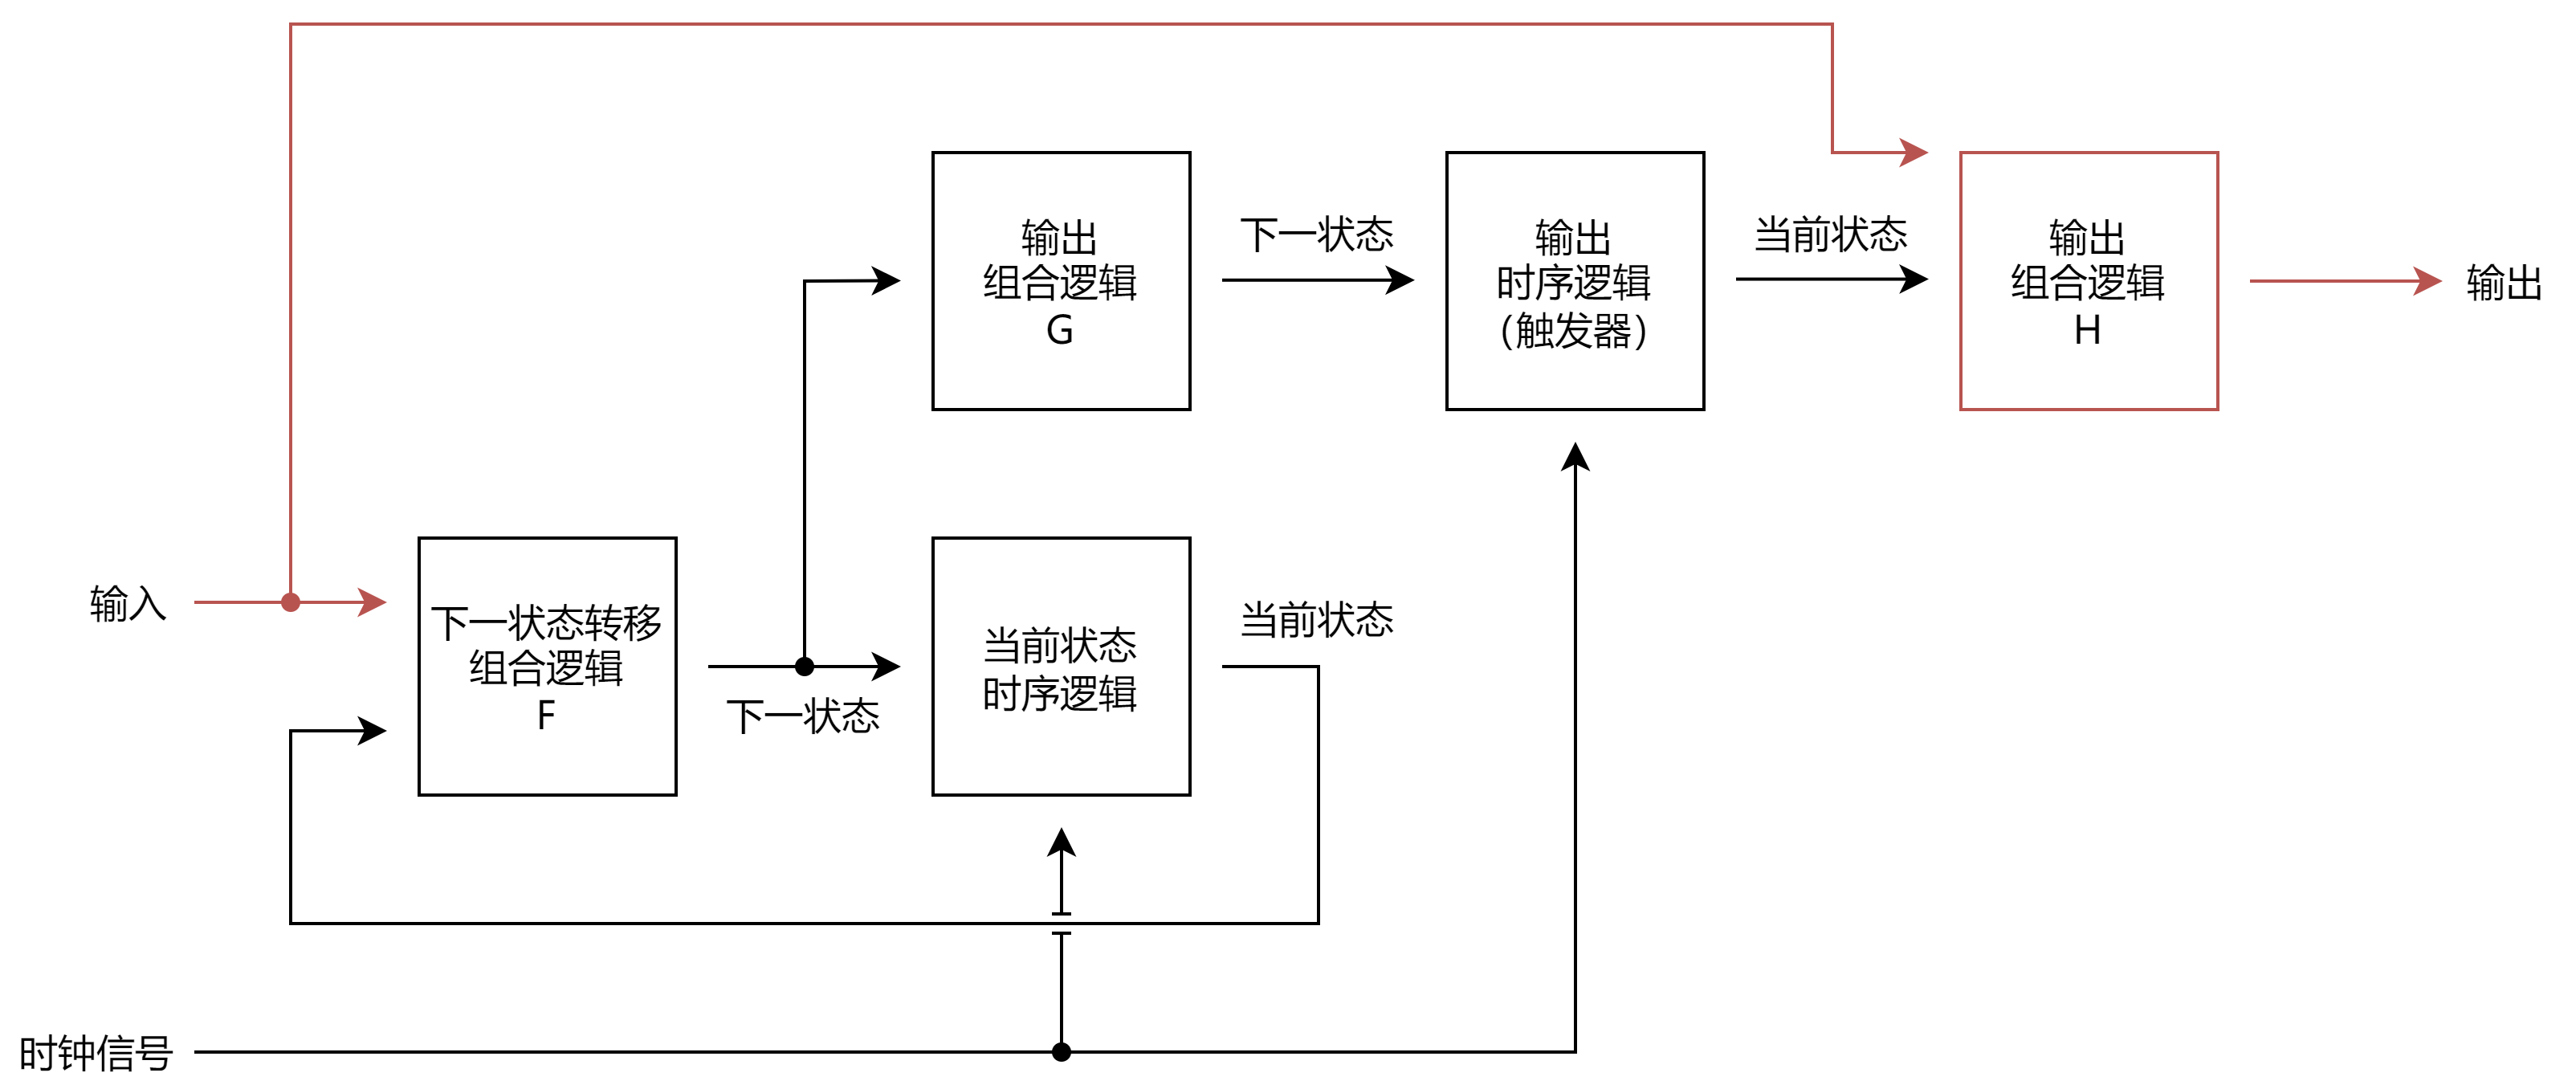
\includegraphics[width=\textwidth]{lab2/8.png}
\end{figure}

这么做显然是与三段式写法的初衷相违背——状态机的输出仍然是组合逻辑驱动的,依然存在产生信号毛刺的可能。因此,\textbf{三段式写法一般仅适用于Moore机}。

%------------------------------%

\section{交通信号灯}

有限状态机的一个实际应用是控制交通信号灯。在这一节中您将实现一个交通信号灯的控制器,它可以控制主街和辅街还有人行道的信号灯。

\subsection{交通信号灯介绍}

本实验中的交通信号灯主要用于控制主街和辅街交汇处的十字路口,两条道路方向上都有红黄绿三色信号灯。下图给出了该十字路口的示意。

\begin{figure}[H]
    \centering
    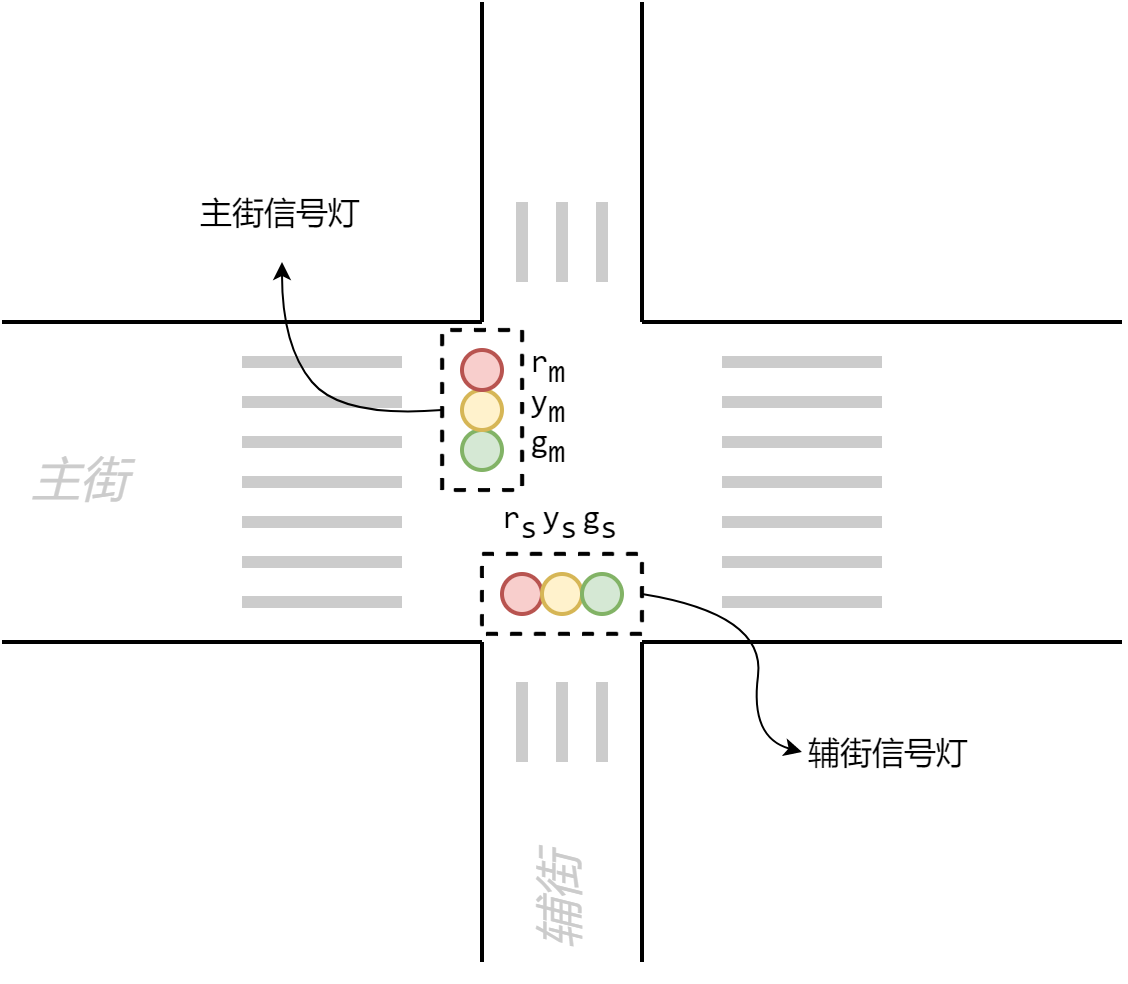
\includegraphics[width=0.5\textwidth]{lab2/9.png}
\end{figure}

\begin{table}[H]
    \centering
    \caption{符号定义}
    \begin{tabular}{ c c c }
        \hline
        变量名称 & 符号 & 默认值(秒)\\
        \hline
        基本时长 & $t_{BASE}$ & 6 \\
        黄灯时长 & $t_{YEL}$ & 2 \\
        \hline
    \end{tabular}
\end{table}

这个十字路口的信号灯开始于主街的绿灯。经过$2 \times t_{BASE}$秒之后,主街信号灯变为黄色。再经过$t_{YEL}$秒之后,主街信号灯变为红色,同时,辅街的信号灯亮起绿色。类似的,辅街的绿色信号灯经过$t_{BASE}$秒之后变为黄色,再经过$t_{YEL}$秒之后变为红色。上述过程不断循环进行。

\subsection{状态机设计}

根据上述的信号灯描述,我们可以简单根据每个信号灯的亮灭画出状态图草图,如下图所示。其中,$R_m, Y_m, G_m$分别表示主街红黄绿灯的亮起状态,$R_s, Y_s, G_s$分别表示辅街红黄绿灯的亮起状态。

\begin{figure}[H]
    \centering
    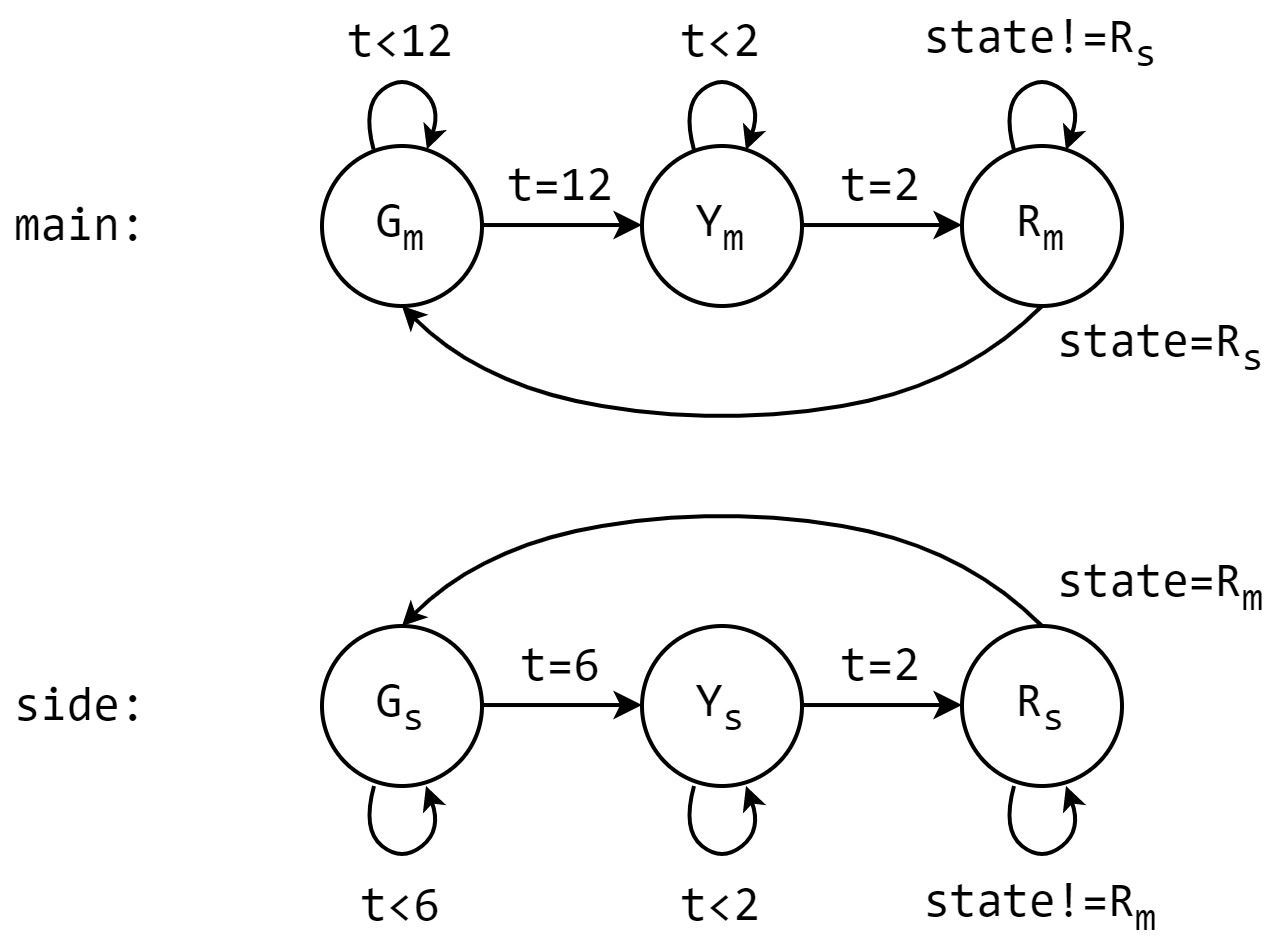
\includegraphics[width=0.5\textwidth]{lab2/10.png}
\end{figure}

由于信号灯的对偶性,主街的红色信号灯一定与辅街的绿色或黄色信号灯同时亮起,而辅街的红色信号灯一定与主街的绿色或黄色信号灯同时亮起。换句话说,一条街的红灯是否亮起,可以根据另一条街的信号灯状态进行判断。因此,进一步地,我们可以减少两个红灯状态以精简状态机,如下图所示。

\begin{figure}[H]
    \centering
    
\includegraphics[width=0.5\textwidth]{lab2/11.png}
\end{figure}

下面我们进行状态赋值,假设目标输出是$[R_m, Y_m, G_m, R_s, Y_s, G_s]$六位二进制信号,用以分别控制主街红黄绿信号灯与辅街红黄绿信号灯的亮灭,高电平时有效。

最简单地,假设我们使用两位二进制00、01、10、11表示4个状态。在输出端,我们则需要一个组合逻辑来表示$[00, 01, 10, 11] \rightarrow [R_m, Y_m, G_m, R_s, Y_s, G_s]$的映射,代码实现较为复杂。

幸运的是,我们定义状态时,使用每个信号灯的亮灭作为状态,而且我们设计的是一个Moore机,这使得简化输出电路成为可能。这里我们直接使用$[R_m, Y_m, G_m, R_s, Y_s, G_s]$六位二进制作为状态,状态机的状态即输出,就不存在输出组合逻辑毛刺的可能,也就不需要使用三段式写法来优化。状态机的状态定义如下。

$$ G_m = 001100_b $$
$$ Y_m = 010100_b $$
$$ G_s = 100001_b $$
$$ Y_s = 100010_b $$

\subsection{状态机实现}

下面我们使用两段式写法来实现这个信号灯的状态机。代码中已经实现了一个计时器,接受1HZ的时钟信号,\underline{在状态转换时计时器归零}。

\textbf{STEP4}:根据信号灯的状态图以及状态赋值,完成以下信号灯状态机的Verilog代码填空,使之实现正确的功能。

\begin{lstlisting}[language=Verilog]
module fsm (
    input CLK1HZ,
    input reset,
    output [3:0] curr_time,
    output [2:0] ryg_main, // red, yellow, green
    output [2:0] ryg_side  // red, yellow, green
);

    parameter Gm = 6'b001100;
    parameter Ym = 6'b010100;
    parameter Gs = 6'b100001;
    parameter Ys = 6'b100010;
 
    reg [3:0] timer;
    always @(posedge CLK1HZ or posedge reset) begin
        if (reset)
            timer <= 4'd0;
        else if (next_state != state)
            timer <= 4'd0;
        else
            timer <= timer + 4'd1;
    end
    assign curr_time = timer;

    // fsm
    
    reg [5:0] next_state;
    reg [5:0] state;
    
    always @(state, timer) begin
        case (state)
            Gm: next_state = timer == 4'd12 ? Ym : Gm;
            Ym: next_state = /***** fill in this field *****/;
            Gs: next_state = /***** fill in this field *****/;
            Ys: next_state = /***** fill in this field *****/;
            default: next_state = Gm;
        endcase
    end

    always @(posedge CLK1HZ or posedge reset) begin
        if (reset)
            state <= Gm;
        else
            state <= next_state;
    end

    assign {ryg_main, ryg_side} = state;

endmodule
\end{lstlisting}

%------------------------------%

\section{上板测试}
我们提供了一个测试模块,用以在FPGAOL平台上或您的开发板上驱动外设。该测试模块的主要功能是:
\begin{itemize}
    \item 使用6个LED展示当前主街和辅街的信号灯亮灭
    \item 使用1位数码管显示当前计数器的数值
    \item 提供按钮复位功能
\end{itemize}

请在您创建的工程项目中导入我们的测试文件(见附件test\_top.v)和相应的约束文件(见附件fpgaol.xdc),并在测试文件中补充您在3.3节中所写信号灯状态机的代码。

所有代码编写完成后,使用Vivado完成代码的\underline{综合、实现、生成比特流}的操作,并将生成的比特流上传到FPGAOL平台或自己的板卡上进行测试。在FPGAOL平台上的展示效果如图所示。

\begin{figure}[H]
    \centering
    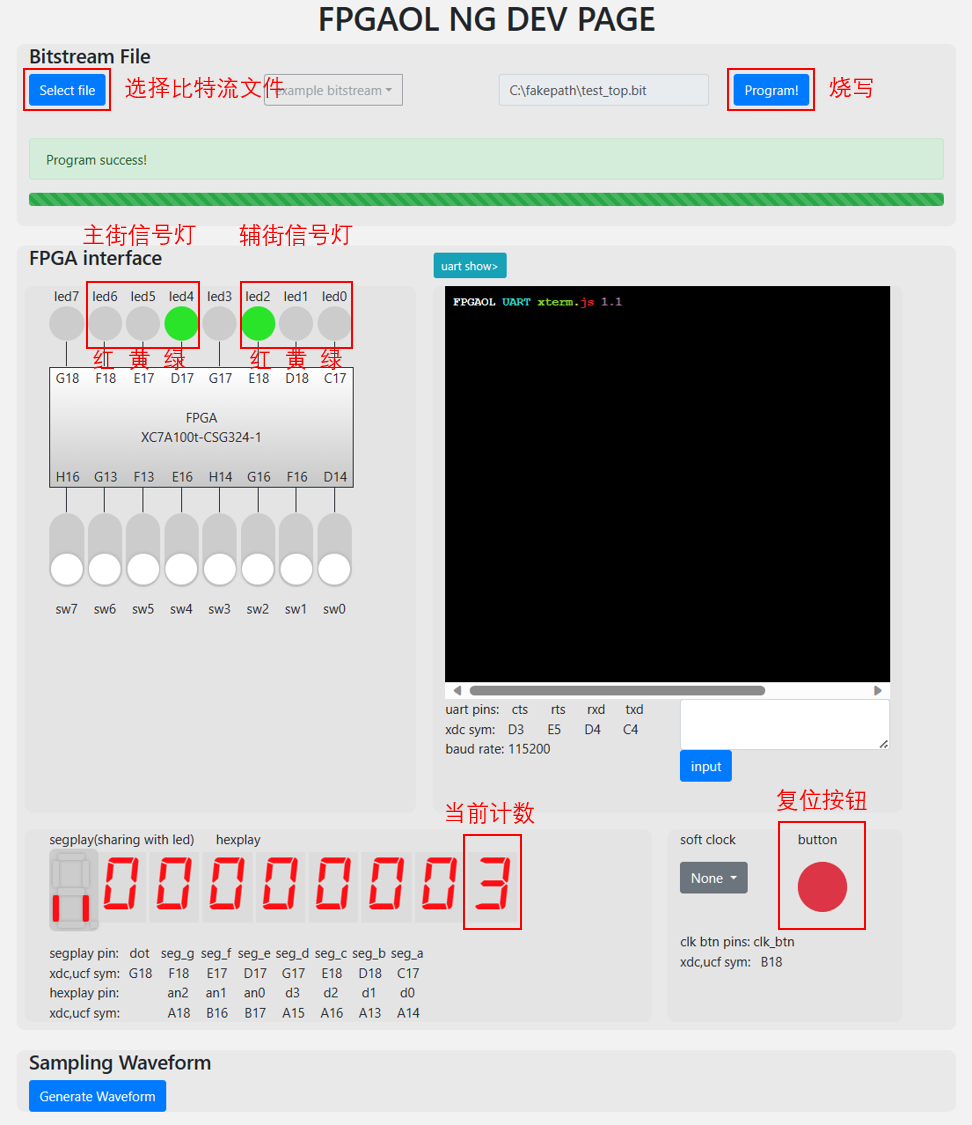
\includegraphics[width=0.65\textwidth]{lab2/12.png}
\end{figure}

%------------------------------%

\section{附件}

\subsection{test\_top.v}

\begin{lstlisting}[language=Verilog]
`timescale 1ns / 1ps

module test_top (
    input CLK100MHZ,
    input reset,
	output reg [2:0] hexplay_an,
	output reg [3:0] hexplay_data,
    output [2:0] ryg_main, // red, yellow, green
    output [2:0] ryg_side  // red, yellow, green
);

    reg [31:0] data;
    reg [32:0] hexplay_cnt;

    always@(posedge CLK100MHZ) begin
        if (hexplay_cnt >= (2000000 / 8))
            hexplay_cnt <= 0;
        else
            hexplay_cnt <= hexplay_cnt + 1;
    end

    always@(posedge CLK100MHZ) begin
        if (hexplay_cnt == 0)begin
            if (hexplay_an == 7)
                hexplay_an <= 0;
            else
                hexplay_an <= hexplay_an + 1;
        end
    end
    
    always@(*) begin
        case(hexplay_an)
            0: hexplay_data = data[3:0];
            1: hexplay_data = data[7:4];
            2: hexplay_data = data[11:8];
            3: hexplay_data = data[15:12];
            4: hexplay_data = data[19:16];
            5: hexplay_data = data[23:20];
            6: hexplay_data = data[27:24];
            7: hexplay_data = data[31:28];
        endcase
    end

    reg [31:0] timer_cnt;
    always@(posedge CLK100MHZ) begin
        if (timer_cnt >= 100000000)
            timer_cnt <= 0;
        else
            timer_cnt <= timer_cnt + 1;
    end

    wire [3:0] curr_time;
    always@(posedge CLK100MHZ) begin
        if (timer_cnt == 0) begin
            data <= curr_time;
        end
    end

    wire CLK1HZ;
    divider u_divider (CLK100MHZ, CLK1HZ);
    fsm u_fsm (CLK1HZ, reset, curr_time, ryg_main, ryg_side);

endmodule

module divider (
    input CLK100MHZ,
    output CLK1HZ
);

    parameter CNT_MAX = 32'd100000000;
    reg [31:0] cnt;
    always @(posedge CLK100MHZ) begin
        if (cnt == CNT_MAX)
            cnt <= 'd0;
        else
            cnt <= cnt + 'd1;
    end
    assign CLK1HZ = cnt == CNT_MAX;
    
endmodule

module fsm (
    input CLK1HZ,
    input reset,
    output [3:0] curr_time,
    output [2:0] ryg_main, // red, yellow, green
    output [2:0] ryg_side  // red, yellow, green
);

    parameter Gm = 6'b001100;
    parameter Ym = 6'b010100;
    parameter Gs = 6'b100001;
    parameter Ys = 6'b100010;

    reg [3:0] timer;
    always @(posedge CLK1HZ or posedge reset) begin
        if (reset)
            timer <= 4'd0;
        else if (next_state != state)
            timer <= 4'd0;
        else
            timer <= timer + 4'd1;
    end
    assign curr_time = timer;

    // fsm
    
    reg [5:0] next_state;
    reg [5:0] state;
    
    always @(state, timer) begin
        case (state)
            Gm: next_state = timer == 4'd12 ? Ym : Gm;
            Ym: next_state = /***** fill in this field *****/;
            Gs: next_state = /***** fill in this field *****/;
            Ys: next_state = /***** fill in this field *****/;
            default: next_state = Gm;
        endcase
    end

    always @(posedge CLK1HZ or posedge reset) begin
        if (reset)
            state <= Gm;
        else
            state <= next_state;
    end

    assign {ryg_main, ryg_side} = state;

endmodule
\end{lstlisting}

\subsection{fpgaol.xdc}
\begin{lstlisting}[language=Verilog]
## Clock signal
set_property -dict { PACKAGE_PIN E3 IOSTANDARD LVCMOS33 } [get_ports { CLK100MHZ }];
create_clock -add -name sys_clk_pin -period 10.00 -waveform {0 5} [get_ports { CLK100MHZ }];

## FPGAOL BUTTON & SOFT_CLOCK

set_property -dict { PACKAGE_PIN B18   IOSTANDARD LVCMOS33 } [get_ports { reset }];

## FPGAOL LED (signle-digit-SEGPLAY)

set_property -dict { PACKAGE_PIN C17 IOSTANDARD LVCMOS33 } [get_ports { ryg_side[0] }];
set_property -dict { PACKAGE_PIN D18 IOSTANDARD LVCMOS33 } [get_ports { ryg_side[1] }];
set_property -dict { PACKAGE_PIN E18 IOSTANDARD LVCMOS33 } [get_ports { ryg_side[2] }];
set_property -dict { PACKAGE_PIN D17 IOSTANDARD LVCMOS33 } [get_ports { ryg_main[0] }];
set_property -dict { PACKAGE_PIN E17 IOSTANDARD LVCMOS33 } [get_ports { ryg_main[1] }];
set_property -dict { PACKAGE_PIN F18 IOSTANDARD LVCMOS33 } [get_ports { ryg_main[2] }];

## FPGAOL HEXPLAY

set_property -dict { PACKAGE_PIN A14 IOSTANDARD LVCMOS33 } [get_ports { hexplay_data[0] }];
set_property -dict { PACKAGE_PIN A13 IOSTANDARD LVCMOS33 } [get_ports { hexplay_data[1] }];
set_property -dict { PACKAGE_PIN A16 IOSTANDARD LVCMOS33 } [get_ports { hexplay_data[2] }];
set_property -dict { PACKAGE_PIN A15 IOSTANDARD LVCMOS33 } [get_ports { hexplay_data[3] }];
set_property -dict { PACKAGE_PIN B17 IOSTANDARD LVCMOS33 } [get_ports { hexplay_an[0] }];
set_property -dict { PACKAGE_PIN B16 IOSTANDARD LVCMOS33 } [get_ports { hexplay_an[1] }];
set_property -dict { PACKAGE_PIN A18 IOSTANDARD LVCMOS33 } [get_ports { hexplay_an[2] }];
\end{lstlisting}

\end{document}